% !TEX root = ../CINTA-cn.tex
%%%%%%%%%%%%%%%%%%%%%%%%%%%%%%%%%%%%%%%%%%%%%%%%%%%%%%%%%%%%%%%%%%%%
% Author: Libin Wang
% Chapter 14. Integer Factorization
% This document was released as open source on 2026-06-18.
% Copyright 2023, Libin Wang. Creative Commons License
% This work is licensed under a Creative Commons Attribution-NonCommercial-NoDerivatives 4.0 International License.
%%%%%%%%%%%%%%%%%%%%%%%%%%%%%%%%%%%%%%%%%%%%%%%%%%%%%%%%%%%%%%%%%%%%

\chapter{整数分解}
\label{chap:factoring} 
\begin{introduction}
  \item 伪多项式时间算法
  \item 大整数分解
  \item Rho 算法
  \item  $p - 1$算法
\end{introduction}

\section{引言}
\label{sec:fac_intr}
之前章节的许多算法都需要对给定的整数求解该整数的素数因子，比如，求欧拉$\varphi$函数的值、求$\Z_p^*$的生成元等，
甚至所有需要使用中国剩余定理的算法都需要使用某个整数的素因子。
本章的核心主题就是：给定一个大整数$n$，如何求出$n$的所有素因子？

以下这种被称为“试除法”的平凡方法广泛用于计算机专业的编程入门练习，相信读者都懂。但是，这是
一种效率不高的算法，不能用于大整数的分解。
\begin{center}
	\lstinputlisting[caption = "整数分解--试除法"]{codes/NaiveFactoring.c}
\end{center}

表面上看，这是一种效率为$\mathcal{O}(\sqrt{n})$的多项式时间算法，为什么说它不高效呢？
其实，这是一种典型的\emph{伪多项式时间}（\emph{pseudo-polynomial time}）算法\index{伪多项式时间}\index{pseudo-polynomial time}。
通常，某些算法对特定的输入值并不感兴趣，而重点关注的是对某一类数值的求解。比如，大整数分解算法并不关心某个特定的整数$n$，而
关心的是$1024$比特这个规模的所有整数的分解。此时，整数分解算法的输入就不是某个整数$n$而是整数$n$的长度$l = \log(n)$，于是
算法的效率就不是$\mathcal{O}(\sqrt{n})$而是$\mathcal{O}(2^{\log(n)/2})$。如果考虑$1024$比特那么长的整数，算法复杂性就具体化为$\mathcal{O}(2^{512})$，
很显然的指数式时间。

SageMath 里面实现了若干整数算法，例子如下，也请大家善于利用它们，以后会用得上。
\begin{example}
\begin{lstlisting}
sage: p = random_prime(2**20); q=random_prime(2**20); n = p*q
sage: factor(n)
628267 * 689713
sage: p = random_prime(2**70); q = random_prime(2**70); n = p*q
sage: qsieve(n)
([71778121402821018943, 833225181856404536623], '')
sage: p = random_prime(2**80); q = random_prime(2**80); n = p*q
sage: time qsieve(n)
CPU times: user 3.05 ms, sys: 8.71 ms, total: 11.8 ms
Wall time: 2.16 s
([746515468832919223969213, 961436815326002097539293], '')
sage: time factor(n)
CPU times: user 670 ms, sys: 93 ms, total: 763 ms
Wall time: 877 ms
746515468832919223969213 * 961436815326002097539293
\end{lstlisting}
\end{example}
以上计算实例从直观上说明，个人计算机分解一两百比特的整数相对较容易，
当然，不是使用上面那个\lstinline{NaiveFactoring} 
算法。
而且，不同的算法效率差异很大，
比如，以上计算实例还显示出，
SageMath 实现的
\lstinline|factor|
算法要比 
\lstinline|qsieve| 
慢很多。

目前最高效的大整数分解工具是\href{http://cado-nfs.gforge.inria.fr/}{Cado-nfs}，它创造了多个分解 RSA 模数的记录，强烈推荐大家下载使用。

目前，尚不存在高效的大整数分解算法。以下介绍的方法只能让读者稍微窥探大整数分解的奥秘。
\section{\texorpdfstring{Pollard 的$p - 1$法}{Pollard 的p - 1法}}
\label{sec:pol_p}

我们介绍的第一种方法是 Pollard 的$p - 1$法，其本质上是一种构造法。
为方便描述，考虑一种非常简洁的大整数$N=pq$，其中$p$和$q$是$N$的两个不相同的素因子。
从一个简单的想法出发：假设可以找到某个整数$m$（也许通过交好运）使得$N$的素因子$p$和$q$（都是未知的值）满足
\[(p-1) \mid m, \text{且}\;(q - 1) \nmid m\]
那么，选取任意的整数$x\in \Z_N^*$，通常取$x = 2$，并计算$y = (x^m - 1) \bmod N$：
\begin{align*}
y &= ((x^m - 1) \bmod N) \leftrightarrow ([(x^m -1)  \bmod p], [(x^m -1) \bmod q])\\
   &= (0, [(x^m -1) \bmod q])
\end{align*}
 
以上计算使用了 CRT 和费尔马小定理。所得的$y$大概率会被$p$整除，但是不被$q$整除。
$y$被$p$整除是因为$m$是$p-1$的倍数，然后根据费尔马小定理即得。
$y$不被$q$整除的理由也很简单，因为任取$x\in \Z_N^*$，$x$以大概率是$\Z_q^*$的生成元。
现在，$ p \mid y$且$p \mid N$。那么，通过使用$\gcd$算法可求出素因子$p$，
即计算$\gcd(y, N)$可得$p$。

接下来再讨论以上思路的几个关键点。首先，怎么样才能找到符合条件的$m$？
如果$p - 1$恰好是某些小素数的乘积（又是一种假设），则$p-1$会整除某个$n!$，$n$是某个不太大的整数值。 
所以，只需要取$m = n!$即可。

但是，即使$n$不大，$n!$也可能是一个巨大的数值。幸运的是，算法只需要模$N$下的计算，
实际上参加计算的数值并不超过$N$。并且，也不需要每次迭代都去
直接计算$(x^{n!} \bmod N)$，因为
\[x^{(n+1)!} \equiv (x^{n!})^{n+1} \pmod{N}\]
算法的实际操作是，对$n = 2, 3, \ldots $不断迭代计算： 
\[ \gcd(((x^{n!} - 1)\bmod N), N)\]
直到计算出一个不为$1$的返回值。
请看算法的具体实现。
%
% \item Furthermore, we can raise the small primes to some power, e.g., given a positive integer $B$, compute:
%\[\prod_{p\in S} p^{\lceil log_p B \rceil} ,\]
%where $S$ contains all the primes up to $B$.
%
%
\begin{center}
	\lstinputlisting[label=alg:p_minus_one_1, caption = Pollard 的$p - 1$法--版本1.]{codes/PollardPM1-2.py}
\end{center}

\begin{example}
令$a=2$，$N=121$。迭代做以下计算：
\begin{enumerate}
\item $a^2 \pmod{N} = 4$
\item $a^3 \pmod{N} = 64$
\item $a^4 \pmod{N} = 82$
\item $a^5 \pmod{N} = 56$
\item $\gcd(56-1, N) = 11$
\end{enumerate} 
得到$11$是$121$的一个素因子。其中，$11-1 = 10 = 2 \cdot 5$，恰好整除$5!$。
\end{example}

%Examples from HPS
\begin{example}
设$a=2$，
\begin{enumerate}
\item 如果$N = 13927189$，则$\gcd(a^{14!} -1, N) = 3823$。这里，$3822 = 2 \cdot 3 \cdot 7^2 \cdot 13$，整除$14!$。

\item 如果$N = 168441398857$，则$\gcd(a^{53!} -1, N) = 350437$。其中，$350436 = 2^2 \cdot 3 \cdot 19 \cdot 29 \cdot 53$，整除$53!$。
\end{enumerate} 
\end{example}

关于$m$的取法，不同的教科书会有稍微不同的做法，
比如不用阶乘，而是使用素数的乘积，那么就需要维护一张素数的列表。在此不再详细讨论，
请看算法~\ref{alg:p_minu_one_2}的具体实现。
\begin{center}
\lstinputlisting[label = alg:p_minu_one_2, caption = Pollard 的$p - 1$法--版本2.]{codes/PollardPM1.py}
\end{center}

Pollard 的$p - 1$法需要一个非常重要的假设：$p - 1$恰好是某些小素数的乘积。如果$p - 1$的素因子都小于等于某个整数$B$，
则称$p - 1$是一个$B$-平滑整数。这是一个值得一提的概念。
如果要分解的大整数$N$不配合表演怎么办？没办法，只能承认，分解失败。换而言之，
$p - 1$法不必然成功。如果成功，其效率还是颇高的，只是$n$次模$N$的指数运算的开销。Pollard 的$p - 1$法告诉我们，
分解整数的开销不仅仅依赖于整数的大小，还依赖整数的本身性质。这是值得强调的事实。

\section{Pollard 的 Rho 算法}
\label{sec:pol_rho}
要理解 Rho 算法，还是从最简单的情形出发。给定一个大整数$N = pq$，$p$和$q$分别是$N$的两个不同的素因子。
如果可以幸运地找到两个整数$x,y \in \Z_N^*$使得$x \equiv y \pmod{p}$成立，则称发生了一次\emph{碰撞}（\emph{collision}）。
当然，不可能同时再有$x \equiv y \pmod q$成立，否则$x$和$y$将大于$N$。
于是使用$\gcd$算法，计算$\gcd(x - y, N)$
则必然得到$N$的某个非平凡的素因子。

如何能求出那两个满足条件的幸运整数$x$和$y$呢？根据生日悖论，如果均匀随机选取$\mathcal{O}(\sqrt{p})$个$\Z_N^*$元素，那么以
很大的概率必然会有两个数发生碰撞。但是，如果只是均匀随机选取$\mathcal{O}(\sqrt{p})$个$\Z_N^*$元素，并对元素两两测试
判断是否一次碰撞，则需$\mathcal{O}(p)$次计算，这并不比试除法好到哪里去。%(k, 2) = \mathcal{O}(k^2)，这里的k是根号p。

\begin{thinking}
上面这个“$\mathcal{O}(p)$次计算”的结论是怎么得到的呢？
\end{thinking}

基于以上观察，Pollard 设计了这样一种方法，使用一个特定的随机函数$F\colon \Z_N^* \to \Z_N^*$，
从某个随机值$x\in \Z_N^*$出发，进行一次包含以下三个过程的\emph{龟兔赛跑}：

\noindent $\bullet$ \textbf{乌龟过程}：这是一次慢计算，
\[x \equiv  F(x) \pmod N\]

\noindent $\bullet$ \textbf{兔子过程}：这是一次快计算，算法开始前，令$x' = x$，
\[x' \equiv  F(F(x')) \pmod N\]

\noindent 之所以称兔子过程是快计算，是因为兔子跑了两步（做了两次$F$函数计算），而乌龟只跑了一步（做了一次$F$函数计算）。 

\noindent $\bullet$ \textbf{计算、判断过程}：计算
\[d = \gcd(x - x', N) \]
如果$d$是一个非平凡因子，则算法结束，返回$d$，否则继续龟兔赛跑过程。

具体算法描述如下：
\begin{center}
	\lstinputlisting[caption = Pollard 的 Rho 算法--通用版本]{codes/GeneralPollardRho.py}
\end{center}

%To do：add a figure.
\iffalse
Pollard 的 Rho 算法用图形直观地表示为图~\ref{fig:PolRho}。

\begin{figure}
\begin{center}
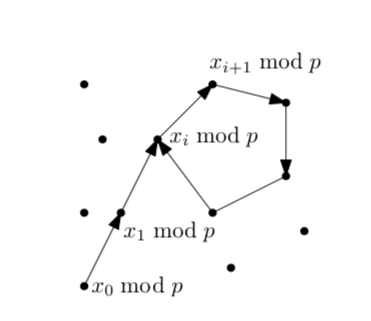
\includegraphics[scale=0.38]{figures/PollardRho.png} 	
\caption{A cycle formed by the tortoise ($x_1$) and the hare ($x_2$) .}
\label{fig:PolRho}       % Give a unique label
\end{center}
\end{figure}

\fi

著名的算法教科书《算法导论》使用以下随机函数：
\[F(x) = x^2 - 1 \pmod{N}\]
并且在满足某个特定条件时，加快兔子的速度，即不总是跑多一步，而是跑$2^k$步，$k$是一个变量。
具体过程见算法~\ref{alg: rho_CLRS}。
\begin{center}
	\lstinputlisting[label = alg: rho_CLRS, caption = "Pollard 的 Rho 算法--算法导论版本."]{codes/PollardRho.py}
\end{center}

以下例子用的是通用 Rho 算法，随机函数定义为$F(x) = x^2 - 1 \pmod{N}$。
\begin{example}
设$N = 77 $，令$x = 51$和$x' = 51$。 
\begin{itemize}
\item \textbf{乌龟过程}：$x = F(x) = 59$；

\item \textbf{兔子过程}：$x' = F(F(x')) = 15$；

\item 计算$\gcd(x - x', N) = 11$。
\end{itemize} 
\end{example}
\begin{example}
设$N = 3013$，令$x = x' = 752 $。 
\begin{itemize}
\item \textbf{乌龟过程}：$x = F(x) $，得到以下数字序列：
\[2072, 2671, 2469, 661, 35, 1224, 714, 598\]
\item \textbf{兔子过程}：$x' = F(F(x')) $，得到以下数字序列：
\[2671, 661, 1224, 598, 2300, 276, 2392, 575\]
\item 最后，$\gcd(598 - 575, N) = 23$，总共迭代了$8$次。
\end{itemize} 
\end{example}

Pollard 的 Rho 算法的期望开销是$\Theta(\sqrt{N})$，依然是一个指数式的复杂度。值得强调，通过碰撞来求解是设计算法的一种常用手段，
在第~\ref{chap:dlog}章我们还会碰到类似的算法。
%How to improve? "Batch gcd" suggested in CLRS.

%%2023年2月8日写
%%2023年6月24日改
\section*{章注}
\addcontentsline{toc}{section}{章注}
以上介绍的整数分解算法被统一归类为\emph{特定目的}（special-purpose）算法，即算法的运行时间依赖于被分解整数的某些属性。
学完本书第~\ref{chap:EC}章后可以理解的\emph{椭圆曲线分解法}（elliptic-curve method，简记为 ECM）也被归类为特定目的算法，
它适合分解的大整数的素因子大概在$50$到$60$个十进制数位范围之内。ECM 是目前运行速度第三快的大整数分解算法。

还有一类算法称为\emph{一般目的}（general-purpose）算法，即算法的运行时间仅仅依赖于被分解整数的大小。目前已知最快和第二快的算法分别是：
\emph{泛数域筛法}（general number field sieve，简记为 GNFS）和\emph{二次筛法}（quadratic sieve）。这两种算法都是亚指数算法，对其进行讲解不属于本书的任务。

由于大整数分解的难解性是 RSA 算法的安全基础，该问题持续成为密码学家关注的重点问题。近年来，对大整数分解的理论突破不多，但是，实践上不断有更多的
RSA 模数被攻破。比如，2020年，RSA250（250位十进制数位，829比特）
被 Cado-nfs 攻破\footnote{出自\href{https://en.wikipedia.org/wiki/RSA_Factoring_Challenge}{维基百科}。}。

\begin{problemset}
\item 请列举若干伪多项式时间（但实际上是指数时间的）算法。

\item 请使用 Pollard 的$p - 1$法对以下整数进行分解：$1537$、$759461789$、$434351781287$。
请指出，所求出的素因子$p$恰好满足$(p-1) \mid n!$时的$n$是多少？

\item 请使用 Pollard 的$p - 1$法分解整数：$132193$。你会有什么奇怪的发现吗？你的发现说明什么呢？
[提示：用其他方法分解$132193$，并找所得素因子之间的关系。]
%https://math.stackexchange.com/questions/3527401/why-is-the-pollards-p-1-method-not-efficient-for-some-numbers
% 132193 = 163*811
% the largest prime power dividing 163−1
% is the same as the largest prime power that divides 811−1
% 20230213，有意思。

\item 请使用 Pollard 的 Rho 算法对以下整数进行分解：$1537$、$759461789$、$434351781287$。
并分别对比 Rho 算法与$p-1$法的运行时间，与所求得的素因子。

\item 设$N = pq$，$p$和$q$是两个不同的素数。如果可以求得一个对$1$模$N$开根号的非平凡解$x$，
即$x^2 \equiv 1 \pmod{N}$，且$x \neq \pm 1$。证明$\gcd(x -1 , N)$和$\gcd(x + 1, N)$都是$N$的非平凡因子。
如果证明成立，似乎找到了一个分解$N$的算法，请问，这样分解$N$的算法复杂度是多少？

\item 设$N = pq$，$p$和$q$是两个不同的素数。如果$p$与$q$的大小非常接近，如何分解$N$？请设计一种算法分解以下特殊的大整数。
\[\bullet 129042418383440439113281876255811982041371046854759858924949\]
\[\bullet 1260424177336333180696659379033392906511175465157564980380984622127793109\]
\noindent 这题在警告我们，并非所有大整数都很难分解。

\item 设$N = pq$，$p$和$q$是两个不同的素数。如果知道$\varphi(N)$，如何分解$N$？提示：利用已知的$N$和$\varphi(N)$构造一个解为$p$和$q$的一元二次方程。
请设计一个算法并编程实现，完成该整数分解过程。

\item Pollard 的$p - 1$法往往对分解大整数表现得无能为力。换一个方向思考，你能不能设计一种算法，构造出总是能被 Pollard 的$p - 1$法高效分解的大整数？
请设计算法并编程实现。
\end{problemset}
